\documentclass[a4paper]{ctexart}
\usepackage{geometry}
\geometry{left=2.5cm,right=2.5cm,top=2.0cm,bottom=2.0cm}

\usepackage{fancyhdr}
\usepackage{graphicx, subfigure}

\usepackage{float}

\usepackage{xcolor}
\IfFileExists{upquote.sty}{\usepackage{upquote}}{}
\usepackage{url}

% \usepackage[sort&compress]{natbib}
\usepackage{hyperref}
\hypersetup{unicode, colorlinks=false, linkcolor=black, urlcolor=blue}
\usepackage{booktabs}
\usepackage{multicol}
\usepackage{amsmath}
\usepackage{pgfplots}
\pgfplotsset{compat=1.15}
\usepackage{mathrsfs}
\usetikzlibrary{arrows}

\definecolor{ffzzqq}{rgb}{1,0.6,0}
\definecolor{qqwuqq}{rgb}{0,0.39215686274509803,0}
\definecolor{xdxdff}{rgb}{0.49019607843137253,0.49019607843137253,1}

\title{\textbf{第三次大作业实验报告}}
\author{
zxdclyz
\and
duskmoon314
\and
BobAnkh
}
\date{December 2020}

\ctexset{
    section = {
      format = \zihao{4}\heiti,
      beforeskip = {2ex},
      afterskip = {2ex}
     },
    subsection = {
            format = \zihao{5}\heiti,
            beforeskip = {2ex},
            afterskip = {1ex},
        },
    subsubsection = {
            format = \zihao{5}\songti,
            beforeskip = {2ex},
            afterskip = {1ex},
        },
    appendix = {
            name = {附录}
        }
}

\linespread{1}

\begin{document}

\pagestyle{plain}

\maketitle

\section{原理介绍}
\subsection{基本思路}
本次实验要求我们根据给出的视频和音频的数据,完成音频分类和视频音频匹配的任务。音频数据为四个壁上的麦克风采集到的声音,我们首先对声音数据进行短时傅里叶变换,将得到的四个特征图作为四个channel,直接使用CNN进行图像分类。而对于匹配问题,我们的想法是根据音频提取出运动相关的一些信息,再与从视频中提取出的相同信息做相似,根据相似度使用KM算法进行匹配,具体选取的特征信息为运动方向和碰撞位置。在本次实验中我们对于视频信息的处理和特征提取是基于传统方法的,我们还设计了基于深度学习的方法(但未将其进行实现),此部分内容详见问题与不足部分。

\centerline{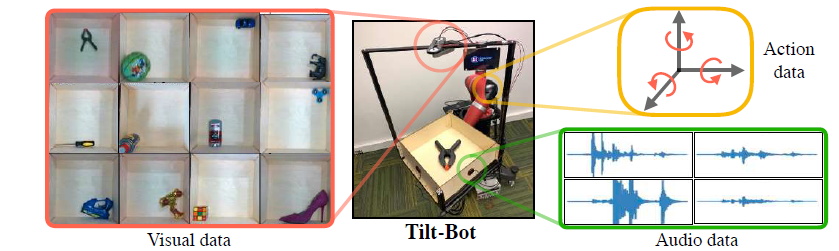
\includegraphics[scale=0.6]{images/dataset.png}}

\subsection{任务一}
首先对音频数据进行预处理,先对音频数据进行降采样(44100Hz$\rightarrow$11000Hz),然后对其进行STFT操作以得到其频谱特征,STFT的具体参数参考了数据集来源的论文\cite{gandhi2020swoosh}。然后对于得到的四个特征图,我们将其当作四个channel拼接为一个tensor,作为训练用的数据。

\centerline{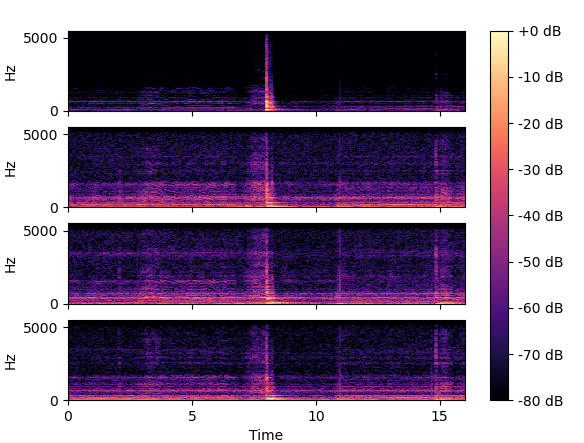
\includegraphics[scale=0.5]{images/audio.png}}

特别的,并不是所有音频数据都是一样长的,绝大多数的音频长度都是4s,对于长度不到4s的音频,我们直接在其末尾使用0进行延拓(padding)。

由于我们得到的训练数据是一个4通道的频谱图,我们可以将其当作一个图像分类任务使用CNN来解决,本次实验中我们使用resnet来解决任务一。
\subsection{任务二、三}
任务二与任务三除了匹配部分没有本质的区别,我们采用的主要思路为先利用类别信息进行分组,然后再在组内进行匹配。对于匹配特征的提取,我们训练了两个网络来分别根据声音判断物体的运动方向和碰撞的位置。事实上,我们认为只根据声音数据,并不能准确恢复出物体的运动方向,因为缺少其开始时的位置信息,因此我们打算使用碰撞位置来作为关键信息进行匹配。但是通过实验发现,许多匹配错误是最终碰撞的位置相同引起的,因此我们加入了并不完全准确的运动方向信息(平均误差在15度)来辅助位置信息进行匹配,从实验结果上看这样的特征组合对匹配成功率有着较为显著的提升。

匹配任务是一个非常典型的二部图最大权匹配,我们采用经典的Kuhn Munkres算法(下称KM算法)来得到匹配结果。考虑到KM算法的时间复杂度较高,先对音频和图像进行较高准确度的分类后,再对每一类内的所有音频和图像信息进行匹配可以有效减少复杂度。如前文所述,音频数据经网络处理后得到“标签-位置-方向”的数据,对图像使用OpenCV处理得到类似的数据。我们将位置和方向拼成一个三维向量$[x, y, \theta]$,并对两份数据的笛卡尔积的每一项都计算两个向量差的二范数的负数作为“匹配度”,即有
\begin{align*}
    S = - \left[(x_1 - x_2)^2 + (y_1 - y_2)^2 + (\theta_1 - \theta_2)^2  \right]
\end{align*}
笛卡尔积使二部图中两部分完全连接,而二范数的负数是为了适应KM算法的最大权匹配的特点。从训练集的实验结果来看,这种方法的可以比较好的对两种数据进行匹配。

\section{具体实现与结果分析}
\subsection{任务一}
基本流程如前所述,先对音频进行了降采样(44100Hz$\rightarrow$11000Hz),然后以参数n\_fft=510, hop\_length=128,对音频进行了stft,这里音频处理使用的库为librosa,与作业二相同。之后我们使用了Resnet-v2\cite{resnet}进行分类任务,通过多次尝试,我们选取了参数较少的resnet20,使用Cross Entropy loss,选用Adma作为优化器,设置初始学习率为1e-3,并在epoch=25, 50, 70对学习率进行0.1的decay。训练和验证的准确率绘制如下,训练了100个epoch,最终训练集上准确率达到98\%,验证集上准确率达到99\%。

\centerline{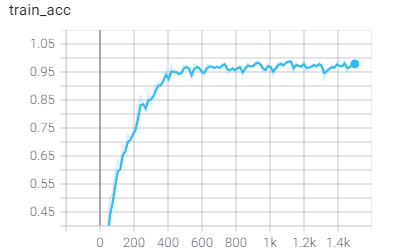
\includegraphics[scale=0.65]{images/audio_train.png}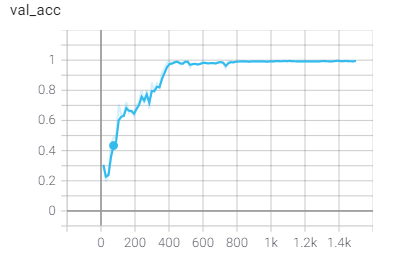
\includegraphics[scale=0.65]{images/audio_cal.png}}
\subsection{任务二、三}

\subsubsection{信息提取}
首先是对音频数据中信息的提取。我们的目标是获取最终的碰撞位置和运动角度的信息,处理的数据与任务一无异,因此我们同样使用Resnet-v2来完成。

对于位置判断,将resnet的输出设为2维,经测试我们选用了resnet110,使用MSE loss,选用Adma作为优化器,设置初始学习率为1e-3,并在epoch=200, 400对学习率进行0.1的decay。训练和验证的loss绘制如下,总共训练了320个epoch,最终训练集上loss达到46,验证集上loss达到613,可见效果虽然不错但还是有一些偏差的。

\centerline{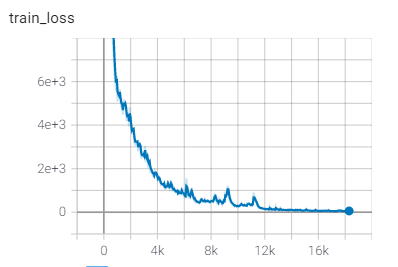
\includegraphics[scale=0.65]{images/loc_train.png}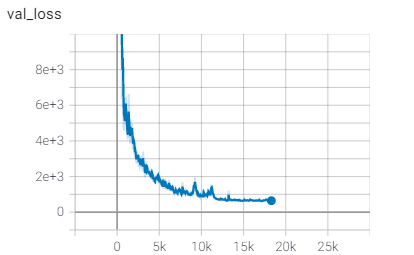
\includegraphics[scale=0.65]{images/loc_val.png}}

对于角度判断也相同,将resnet的输出设为1维即可,我们同样使用resnet110,使用MSE loss,选用Adma作为优化器,设置初始学习率为1e-3,并在epoch=200, 400对学习率进行0.1的decay。这里我们定义了两个角度差的cos值作为相似度来评判模型训练的好坏,经过500epoch的训练,最终训练集上相似度达到0.99,验证集上相似度达到0.96,0.96对应平均有16度的误差,如此大的误差已经会影响到我们进行匹配,因此我们没有选择角度作为唯一特征。

\centerline{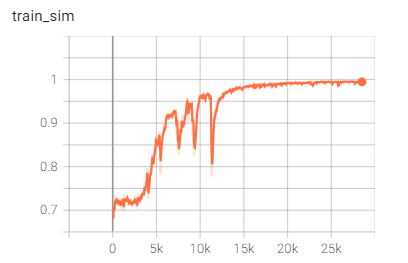
\includegraphics[scale=0.65]{images/angle_train.png}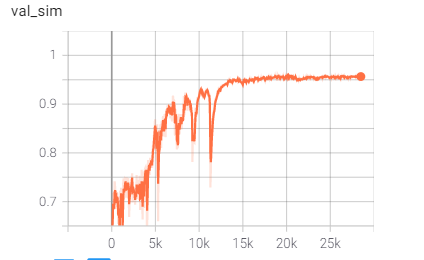
\includegraphics[scale=0.65]{images/angle_val.png}}

其次是对于图像的处理,为了与音频信息计算相似度,图像也同样需要碰撞位置和运动角度信息,同时还需要对图像进行分类来与音频先进行一个粗匹配。

对图像的分类十分简单,依然使用Resnet-v2完成。选取resnet44,使用Cross Entropy loss,选用Adma作为优化器,设置初始学习率为1e-3,并在epoch=20, 40对学习率进行0.1的decay。训练和验证的准确率绘制如下,仅训练了50个epoch,训练集和验证集上准确率均达到100\%。

\centerline{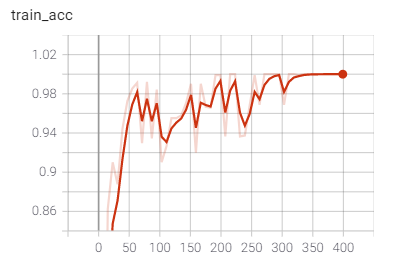
\includegraphics[scale=0.65]{images/image_train.png}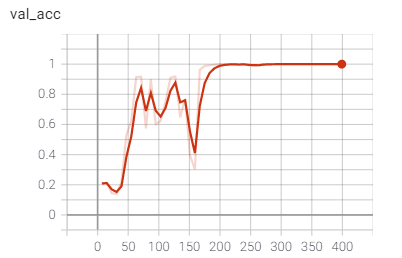
\includegraphics[scale=0.65]{images/image_val.png}}

从图像中提取碰撞位置和运动角度信息的任务使用传统方法完成。使用掩膜图像计算了其各阶矩,图像中心位置可由一阶矩除以零阶矩得到,从而根据最后一张图像得到碰撞位置,由始末两张图像得到其运动角度。

\subsubsection{匹配计算}

我们以Github上开源的KM算法\cite{KM}为基础,并更改KM算法过程中权值的更新以适配负的权值,增加一个入口函数以适配网络给出的预测结果。由于KM算法本身的特性会尽可能的将二部图匹配起来,这便要求输入的音频数据和图像数据数量尽可能接近。同时为了避免无连接时的0导致的问题,也为了增大准确度,我们使用笛卡尔积将邻接矩阵完全填满。实验表明这种做法提升了匹配的结果。

在匹配权重的选择上,我们尝试了单独以位置或角度为权重,在训练集上的最好结果不超过65\%。而使用二者结合后的二范数显著提高了准确率。我们认为后一种方法可以拉开正确匹配与错误匹配间权重的差别,既提升了匹配的正确率,也减小了KM算法更新的次数。

由于数据集本身较小,在完全划分足够测试匹配准确度的验证集的情况下训练数据会减少很多,我们只能在整个数据集上直接划分出一小块来进行匹配的准确度测试,在划分出的50个样本中(每个类别各5个),我们达到了48/50的匹配准确度,并且我们发现匹配出错的原因主要在于音频分类不准确,所以我们有理由认为对于每个类别中较少的需要匹配的个体,我们设计的基于角度、位置信息的相似度计算算法可以较好地完成匹配任务。

\section{问题与不足}
\subsection{目前的问题}
\begin{enumerate}
    \item 我们目前对于视频信息的利用还是比较少的,只用到了初始和最终的两张图来做简单的特征工程,对于我们这次简单的匹配任务还算应付地来,但显然对于其中信息仍可以做到更好地提取以实现更好的效果。
    \item 没有充分检验整个算法的有效性。
    \item KM算法使用的相似度在部分数据间差别较小,还有进一步优化的空间。
\end{enumerate}
\subsection{优化的设计}
\begin{itemize}
    \item 对于视频信息的处理,我们最初的设计是使用ConvLSTM来进行embedding提取信息,对应的,对于音频的处理我们也打算使用embedding的方式来进行,但这样的方式比较有研究意义而对本次实验的帮助可能并不直接,并且调试起来比较耗时,于是我们没有采取这一方案,但我们认为这样的思路对于这一数据集的利用是有帮助的。
\end{itemize}
\section{使用说明与文件清单}

\subsection{使用说明}
\begin{enumerate}

    \item 运行\texttt{setup.py}来安装需要的依赖包。

    \item 确保\texttt{test.py}文件与\texttt{src}文件夹和\texttt{weights}文件夹处于同一级目录下。
    
    注:\textbf{测试需在GPU环境中运行}。另外由于不确定测试设备性能,所以各个dataloader都设置了较小的batchsize,如有需要可自行调大该数值。

\end{enumerate}
\subsection{文件清单}

\begin{table}[H]
    \centering
    \begin{tabular}{ll}
        \toprule
        文件名称         & 说明                       \\
        \midrule
        test.py          & 测试所用主程序  \\
        setup.py         & Python 3.7下配置运行环境  \\
        requirements.txt & 依赖库说明文件                   \\
        train.py     & 训练所用主程序  \\
        src/audio\_process.py     & 预处理audio数据  \\
        src/dataloader.py     & 定义dataset  \\
        src/image\_center.py     & 处理video数据  \\
        src/\_\_init\_\_.py       \\
        src/KM.py     & KM匹配算法  \\
        src/model.py     & 定义各任务所使用的神经网络模型  \\
        weights     & 存放模型权重参数的文件夹 \\

        \bottomrule
    \end{tabular}
\end{table}

\section{成员分工}
模型的设计、报告的编写由三人共同合作完成,其余主要分工如下:
\begin{itemize}
    \item ***:音频数据处理,模型的实现与训练
    \item ***:视频数据处理,模型的实现与训练
    \item ***:匹配算法的实现,dataset和dataloader编写
\end{itemize}
\bibliographystyle{plain} 
\bibliography{ref}
\end{document}
